\chapter{Biological Background}\label{chap:biointro}

In this chapter, we provide a biological background for this work.
We define a genome, describe a DNA sequencing process, and its issues. Then we explain an DNA assembling process, its problems and why it is often not possible to fully assemble the genome.

\section{The Genome}

Each life form is build from at least one cell. One of the most important part of the cell is \emph{DNA (Deoxyribonucleic acid)}, which is located in the cell core.
DNA carries the genetic information used for development, functioning and reproduction of the cell or an organism.
DNA is composed of two complementary strains which form a double helix structure. Each strain consist of many nucleotides, which are one of: cytosine (C), guanine (G), adenine (A), or thymine (T).
The pairs of nucleotides A---T and C---G are complementary, i.e.\ if in one strain there is A in the other is T, and if in one is G in the other is C, see Figure~\ref{fig:dnahelix}.
DNA molecules are organized in chromosomes.
The \emph{genome} is a set of all chromosomes in the cell, it includes both the coding and the non-coding parts of DNA.\@
The coding part of the genome is called gene. Each gene can be translated into a protein sequence which it encodes.

\begin{figure}[htbp]
  \centering
  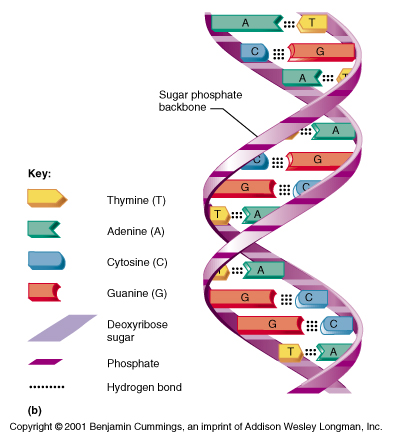
\includegraphics[width=.5\textwidth]{../figures/dna-helix}
  \caption[DNA double helix]{The DNA double helix. Each strain consists of many nucleotides. The nucleotides A---T, and C---G are complementary~\cite{dnahelix}.}\label{fig:dnahelix}
\end{figure}

\section{DNA Sequencing}

Obtaining a DNA sequence or its part from the cell is called \emph{DNA sequencing}.
DNA sequencing connects experimental methods of obtaining the sequence from the cell core and the computational analysis of the sequencing data called sequence assembling.

The first sequenced genome was a simple RNA virus in 1976. The 3.2Gb long human genome was first sequenced in 2001, and it took 13 years and cost about 3 billions dollars. Nowadays it is possible to sequence such large genome for much lower cost (several tens thousands dollars).

The traditional sequencing method, called \emph{Sanger sequencing}, was developed by Frederick Sanger in 1977~\cite{sanger1977dna}. It was used in the first human genome sequencing.
In the Sanger sequencing, a two strand DNA is first split into the single strand DNA.\@ The single strand DNA can be used to create its copies, if particular enzymes and sufficient amount of nucleotides is available. The key role in Sanger sequencing form modified nucleotides. The nucleotides are modified in two ways: they are colored by a florescent coloring and modified, so the DNA copy process cannot continue after the nucleotide. This results in bunch of DNA segments of various lengths, which are the sequenced DNA prefixes interrupted by the colored nucleotide in its last position. Every position is represented by multiple segments. The segments are then sorted by length using electrophoresis, and the colors are read from the shortest to the longest segment, forming a DNA sequence (Figure~\ref{fig:sanger}).

\begin{figure}[htbp]
  \centering
  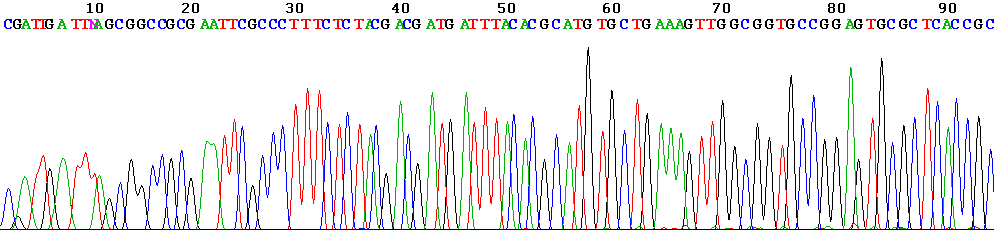
\includegraphics[width=\textwidth]{../figures/sanger}
  \caption[Sanger sequencing]{Example of a Sanger sequencing read. The four bases are detected using different fluorescent labels. These are detected and represented as `peaks' of different colors, which can then be interpreted to determine the base sequence, shown at the top~\cite{wiki:sanger-img}.}\label{fig:sanger}
\end{figure}

Only short sequences, up to 500--1000 bases, can be read this way. Therefore the original DNA has to be split into many overlapping short sequences.
Therefore instead of one long sequence per chromosome, we get many short sequences, which have to be assembled together to obtain the whole sequence.

Since 2005, sequencing machines of the second generation (or the new generation sequencing machines) have been commercially available. There are multiple different technologies for NGS, but they all share some properties.
They produce a huge amount of reads from the same sample, and are faster and cheaper. They also produce much shorter reads (35--400 bases) then the Sanger sequencing, which makes a DNA assembly even harder task.

\section{DNA Assembly}

The DNA assembling aims to construct a whole DNA sequence from short sequencing reads. Ideally, we would get a single sequence per chromosome. In reality, there are usually several problems causing the final sequence to be split into multiple contigs.

The first aspect, which influence the final sequence assembly quality is a coverage of input data. The coverage is an average number of reads covering a single base in the genome (see Chapter~\ref{chap:genomesize} for more details).
As the bases are not covered uniformly, some of the bases may not be covered at all. Those bases are then missing from the assembly and causing the final sequence to be cut at that place. With increasing coverage, the probability that a base would not be covered decreases.
Moreover, the reads may contain errors and the final sequence is built as consensus sequence, in which each base is computed as a consensus from all reads overlapping the base. If a base is covered with very few reads, it may happen, that there are more erroneous bases in the particular position in the reads. Again, with increasing coverage, the probability that this happen decreases. Thus, the higher the coverage, the better the quality of the sequence.

The other problem of the DNA assembling is caused by repetitive sequences. These sequences are often longer than the read length. Thus, there may be several reads from different parts of the repetitive sequence, which may look very similar, and are hard to distinguish. If such repeats occur in tandem, it is then very hard to find out the correct length of the sequence. If the repeats occur randomly in the genome, it may be hard to find out the order of the parts of genome which lay between the occurrences.

There are two main approaches to the genome assembly used in modern genome assemblers. The first is based on overlap-layout-consensus framework (e.g.\ Celera~\cite{myers2000celera}, SGA~\cite{simpson2010sga}). The second is based on de Bruin graphs~\cite{deBruijn} (e.g.\ Velvet~\cite{zerbino2008velvet}, ALLPATHS-LG~\cite{gnerre2011allpaths}). Both this methods construct a string graph~\cite{myers2005stringgraph} from the sequencing data. The first method does it by computing all overlaps, whereas the second method builds it from the de Bruin graph.

Let us consider a genome with several perfect repeats, which lengths are longer then reads. The string graph of a genome is then created by collapsing all the like repetitive sequences (Figure~\ref{fig:string-graph}). If we build a string graph from data, the vertices are all unambiguous sequences, and the edges are between those which are overlapping. An Euler tour in a string graph forms a possible assembly.

\begin{figure}[htbp]
  \centering
  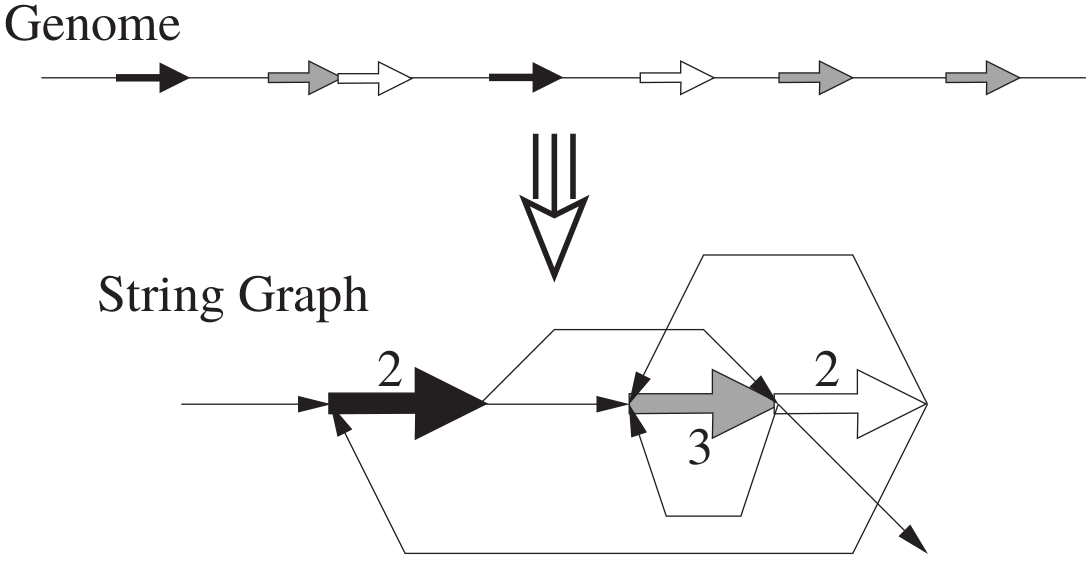
\includegraphics[width=0.5\textwidth]{../figures/string-graph.png}
  \caption[String graph]{A string graph constructed from a genome. The repetitive parts are collapsed together~\cite{myers2005stringgraph}.}\label{fig:string-graph}
\end{figure}

To resolve a repetitive sequence lengths and order of the parts of genome, some assemblers  (e.g.\ ALLPATHS-LG~\cite{gnerre2011allpaths}) use paired reads, which can be obtained from the NGS machines, as additional data. The paired reads are pairs of reads, for which we know approximate distance in the genome. Multiple distance paired reads can be combined together, to get better result.
